\chapter{Komponentit ja virittävät puut}

Tähän mennessä olemme tarkastelleet verkkoja,
joiden rakenne säilyy samana koko algoritmin ajan.
Mitä tapahtuu sitten, jos verkkoon tuleekin \emph{muutoksia},
kuten lisäämme verkkoon uusia kaaria?

Tutustumme tässä luvussa union-find-rakenteeseen,
joka on hyödyl\-linen työkalu verkkojen käsittelyssä.
Rakenteen avulla voimme pitää kirjaa verkon yhtenäisistä
komponenteista ja päivittää rakennetta tehokkaasti,
kun lisäämme verkkoon kaaria.
Voimme esimerkiksi tarkkailla, montako yhte\-näistä
komponenttia verkossa on milläkin hetkellä.

Käsittelemme myös pienimmän virittävän puun ongelmaa,
jossa haluamme kytkeä verkon solmut toisiinsa kaaria käyttäen niin,
että kaarten yhteispaino on pienin.
Voimme ratkaista ongelman tehokkaasti Kruskalin algoritmilla,
joka perustuu union-find-rakenteeseen,
tai Primin algoritmilla, joka muistuttaa Dijkstran algoritmia.

\section{Union-find-rakenne}

Union-find-rakenne on tietorakenne, joka
pitää yllä kokoelmaa alkioiden joukkoja ja tarjoaa
seuraavat tehokkaat operaatiot:

\begin{itemize}
\item yhdistä kaksi joukkoa samaksi joukoksi
\item tarkista, ovatko kaksi alkiota samassa joukossa
\end{itemize}

Oletamme, että alkiot ovat $1,2,\dots,n$,
ja jokainen alkio kuuluu tarkalleen yhteen joukkoon.
Esimerkiksi kun $n=8$, joukot voivat olla vaikkapa
$A=\{1,4\}$, $B=\{2,5,6\}$ ja $C=\{3,7,8\}$.
Kun yhdistämme sitten joukot $A$ ja $B$,
niistä syntyy joukko $\{1,2,4,5,6\}$.
Ennen yhdistämistä alkiot $1$ ja $2$ olivat eri joukoissa,
mutta järjestämisen jälkeen ne ovat samassa joukossa.

\subsection{Rakenteen toteutus}

Toteutamme union-find-rakenteen niin, että jokaisessa joukossa
yksi alkioista on joukon \emph{edustaja} ja muut alkiot viittaavat
edustajaan suoraan tai muiden alkioiden kautta.
Kun haluamme tarkastaa, ovatko kaksi alkiota samassa joukossa,
selvitämme niiden edustajat ja vertaamme niitä toisiinsa.

Jokaisella joukon alkiolla $x$ on arvo $\texttt{seuraava}[x]$,
joka kertoo seuraavan alkion viittauksien ketjussa.
Jos $\texttt{seuraava}[x]=x$, alkio on joukon edustaja.
Tämän ansiosta saamme selville mille tahansa alkiolle $x$,
mikä on vastaavan joukon edustaja, kulkemalla läpi viittausten ketjun.

\begin{figure}
\center
\begin{center}
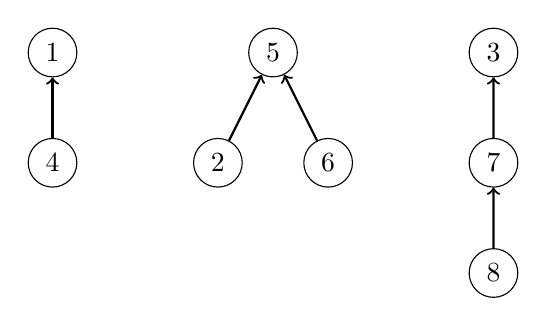
\begin{tikzpicture}[scale=0.7]
\node[draw, circle] (1) at (0,0) {$1$};
\node[draw, circle] (4) at (0,-2) {$4$};

\node[draw, circle] (2) at (3,-2) {$2$};
\node[draw, circle] (5) at (4,0) {$5$};
\node[draw, circle] (6) at (5,-2) {$6$};

\node[draw, circle] (3) at (8,0) {$3$};
\node[draw, circle] (7) at (8,-2) {$7$};
\node[draw, circle] (8) at (8,-4) {$8$};

\path[draw,thick,->] (4) -- (1);
\path[draw,thick,->] (2) -- (5);
\path[draw,thick,->] (6) -- (5);
\path[draw,thick,->] (7) -- (3);
\path[draw,thick,->] (8) -- (7);
\end{tikzpicture}
\end{center}
\caption{Union-find-rakenne joukoille $\{1,4\}$, $\{2,5,6\}$ ja $\{3,7,8\}$.}
\label{fig:unifin}
\end{figure}

Kuvassa \ref{fig:unifin} on union-find-rakenne,
joka vastaa joukkoja $A=\{1,4\}$, $B=\{2,5,6\}$ ja $C=\{3,7,8\}$.
Tässä tapauksessa joukkojen edustajat ovat 1, 5 ja 3.
Esimerkiksi $\texttt{seuraava}[1]=1$, koska alkio $1$ on joukon edustaja,
ja $\texttt{seuraava}[2]=5$, koska alkio $2$ osoittaa alkioon $5$.
Saamme selville, mikä on alkion 8 joukon edustaja, kulkemalla ketjua
$8 \rightarrow 7 \rightarrow 3$.

Seuraava operaatio \texttt{edustaja} selvittää alkion $x$ joukon edustajan:

\begin{code}
int edustaja(int x) {
    while (x != seuraava[x]) {
        x = seuraava[x];
    }
    return x;
}
\end{code}

Tämän avulla voimme luoda operaation \texttt{sama}, joka tarkastaa,
ovatko alkiot $a$ ja $b$ samassa joukossa.
Alkiot ovat samassa joukossa täsmälleen silloin, kun niillä
on sama edustaja:

\begin{code}
boolean sama(int a, int b) {
    return edustaja(a) == edustaja(b);
}
\end{code}

\subsection{Tehokas yhdistäminen}

Viimeinen tarvittava operaatio on \texttt{yhdista}, joka yhdistää alkioita
$a$ ja $b$ vastaavat joukot.
Tämän operaation toteutus ratkaisee, kuinka tehokas rakenteemme on.
Haluamme, että alkioiden viittausten ketjut ovat lyhyitä,
jotta pystymme selvittämään nopeasti alkioiden edustajia.
Saavutamme tämän tavoitteen asettamalla \emph{pienemmän} joukon
edustajan osoittamaan \emph{suuremman} joukon edustajaan.
Jos joukot ovat yhtä suuria, voimme toteuttaa yhdistämisen
kummin päin vain haluamallamme tavalla.

\begin{figure}
\center
\begin{center}
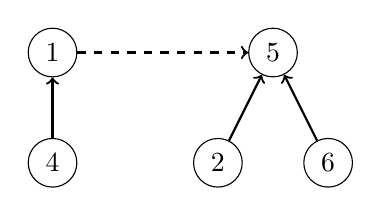
\begin{tikzpicture}[scale=0.7]
\node[draw, circle] (1) at (0,0) {$1$};
\node[draw, circle] (2) at (0,-2) {$4$};
\node[draw, circle] (3) at (4,0) {$5$};
\node[draw, circle] (4) at (3,-2) {$2$};
\node[draw, circle] (5) at (5,-2) {$6$};
\path[draw,thick,->] (2) -- (1);
\path[draw,thick,->] (4) -- (3);
\path[draw,thick,->] (5) -- (3);
\path[draw,thick,->,dashed] (1) -- (3);
\end{tikzpicture}
\end{center}
\caption{Tehokas yhdistäminen. Alkion $1$ joukon koko on 2
ja alkion $5$ joukon koko on 3,
joten yhdistämme alkion 1 alkioon 5.}
\label{fig:tehyhd}
\end{figure}

Kuva \ref{fig:tehyhd} näyttää, mitä tapahtuu, kun yhdistämme joukot
$A=\{1,4\}$ ja $B=\{2,5,6\}$.
Joukon $A$ edustaja on $1$ ja joukon $B$ edustaja on $5$.
Koska joukko $A$ on pienempi, asetamme joukon $A$
edustajan osoittamaan joukon $B$ edustajaan.
Tämän jälkeen kaikki alkiot kuuluvat samaan joukkoon ja
alkio $5$ on tästä lähtien koko joukon edustaja.

Jotta voimme toteuttaa yhdistämisen tehokkaasti,
meidän täytyy myös pitää kirjaa kunkin joukon koosta.
Seuraavassa toteutuksessa $\texttt{koko}[x]$ kertoo,
montako alkiota alkion $x$ edustama joukko sisältää.
Selvitämme ensin joukkojen edustajat ja yhdistämme sitten joukot.

\begin{code}
void yhdista(int a, int b) {
    a = edustaja(a);
    b = edustaja(b);
    if (koko[a] < koko[b]) {
        seuraava[a] = b;
        koko[b] += koko[a];
    } else {
        seuraava[b] = a;
        koko[a] += koko[b];
    }
}
\end{code}

Kun toteutamme yhdistämiset tällä tavalla, jokainen
alkioiden ketju sisäl\-tää vain $O(\log n)$ alkiota.
Tämä johtuu siitä, että aina kun kuljemme ketjussa
askeleen eteenpäin alkiosta $a$ alkioon $b$,
$\texttt{koko}[b] \ge 2 \cdot \texttt{koko}[a]$ eli
edustajaa vastaavan joukon koko ainakin \emph{kaksinkertaistuu}.
Koska joukossa on enintään $n$ alkiota,
kuljemme siis yhteensä enintään $O(\log n)$ askelta.
Niinpä operaatio \texttt{edustaja} toimii ajassa $O(\log n)$,
ja sen myötä myös operaatiot \texttt{sama} ja \texttt{yhdista}
toimivat ajassa $O(\log n)$.

\subsection{Ketjun tiivistäminen}

Pystymme saamaan union-find-rakenteen vielä tehokkaammaksi
toteuttamalla \texttt{edustaja}-operaation seuraavasti:

\begin{code}
int edustaja(int x) {
    return seuraava[x] = edustaja(x);
}
\end{code}

Tässä ideana on \emph{tiivistää} ketjua samalla,
kun kuljemme eteenpäin ketjussa.
Asetamme jokaisen ketjun alkion \texttt{seuraava}-arvoksi sen edustajan,
minkä ansiosta pääsemme suoraan edustajaan,
jos kuljemme samaa ketjua myöhemmin.
Kuva \ref{fig:poltii} näyttää esimerkin ketjun tiivistämisestä.
Kuljemme aluksi ketjua $4 \rightarrow 3 \rightarrow 2 \rightarrow 1$,
jolloin kaikki alkiot asetetaan viittaamaan edustajaan $1$.
Kun haluamme selvittää seuraavan kerran alkion $4$ edustajan,
pääsemme suoraan alkiosta $4$ edustajaan $1$.

\begin{figure}
\center
\begin{center}
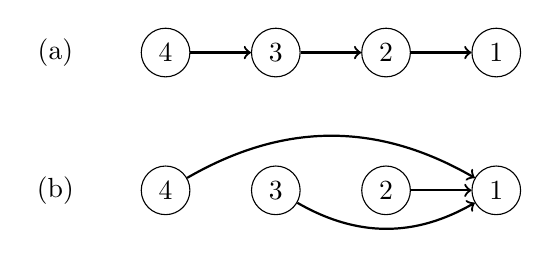
\begin{tikzpicture}[scale=0.7]
\begin{scope}
\node[draw, circle] (1) at (0,0) {$1$};
\node[draw, circle] (2) at (-2,0) {$2$};
\node[draw, circle] (3) at (-4,0) {$3$};
\node[draw, circle] (4) at (-6,0) {$4$};
\path[draw,thick,->] (4) -- (3);
\path[draw,thick,->] (3) -- (2);
\path[draw,thick,->] (2) -- (1);
\node at (-8,0) {(a)};
\end{scope}
\begin{scope}[yshift=-2.5cm]
\node[draw, circle] (1) at (0,0) {$1$};
\node[draw, circle] (2) at (-2,0) {$2$};
\node[draw, circle] (3) at (-4,0) {$3$};
\node[draw, circle] (4) at (-6,0) {$4$};
\path[draw,thick,->] (4) edge [bend left] (1);
\path[draw,thick,->] (3) edge [bend right] (1);
\path[draw,thick,->] (2) -- (1);
\node at (-8,0) {(b)};
\end{scope}
\end{tikzpicture}
\end{center}
\caption{Ketjun tiivistäminen. (a) Alkuperäinen ketju $4 \rightarrow 3 \rightarrow 2 \rightarrow 1$.
(b) Tiivistetty ketju, jossa kaikki alkiot viittaavat suoraan edustajaan.}
\label{fig:poltii}
\end{figure}

On mahdollista osoittaa, että ketjujen tiivistämisen ansiosta
$\texttt{edustaja}$-ope\-raatiot vievät tasoitetusti aikaa vain
$O(\alpha(n))$, missä $\alpha(n)$ on hyvin hitaasti kasvava
\emph{käänteinen Ackermannin funktio}.
Funktiosta tiedetään, että $\alpha(n)<5$, kun $n$ on mikä tahansa
käytännössä esiintyvä joukon koko.
Tämä tarkoittaa, että voimme ajatella union-find-rakenteen
operaatioiden olevan käytännössä \emph{vakioaikaisia}.
Tämän tuloksen osoittaminen on kuitenkin vaikeaa,
emmekä käsittele asiaa tarkemmin tällä kurssilla.

\section{Esimerkki: Kaupungit}

Bittimaassa on $n$ kaupunkia, joiden välillä ei ole vielä yhtään tietä.
Sitten teitä aletaan rakentaa yksi kerrallaan, yhteensä $m$ tietä.
Jokainen tie yhdistää kaksi kaupunkia toisiinsa.
Minkä tien rakentamisen jälkeen kaikki kaupungit ovat ensimmäistä
kertaa yhteydessä toisiinsa?

\begin{figure}
\center
\begin{center}
\begin{tikzpicture}[scale=0.7,label distance=-1.5mm]
\small
\newcommand\verkko[6]{
\node[draw, circle] (1) at (0,-1) {$1$};
\node[draw, circle] (2) at (2,0) {$2$};
\node[draw, circle] (3) at (2,-2) {$3$};
\node[draw, circle] (4) at (4,0) {$4$};
\node[draw, circle] (5) at (4,-2) {$5$};
\node at (2,-3.5) {vaihe #1};
}
\begin{scope}
\verkko{1}
\path[draw,thick,-] (1) -- (2);
\end{scope}
\begin{scope}[xshift=6.5cm]
\verkko{2}
\path[draw,thick,-] (1) -- (2);
\path[draw,thick,-] (1) -- (3);
\end{scope}
\begin{scope}[xshift=13cm]
\verkko{3}
\path[draw,thick,-] (1) -- (2);
\path[draw,thick,-] (1) -- (3);
\path[draw,thick,-] (2) -- (3);
\end{scope}
\begin{scope}[yshift=-5.5cm]
\verkko{4}
\path[draw,thick,-] (1) -- (2);
\path[draw,thick,-] (1) -- (3);
\path[draw,thick,-] (2) -- (3);
\path[draw,thick,-] (4) -- (5);
\end{scope}
\begin{scope}[yshift=-5.5cm,xshift=6.5cm]
\verkko{5}
\path[draw,thick,-] (1) -- (2);
\path[draw,thick,-] (1) -- (3);
\path[draw,thick,-] (2) -- (3);
\path[draw,thick,-] (4) -- (5);
\path[draw,thick,-] (2) -- (4);
\end{scope}
\begin{scope}[yshift=-5.5cm,xshift=13cm]
\verkko{6}
\path[draw,thick,-] (1) -- (2);
\path[draw,thick,-] (1) -- (3);
\path[draw,thick,-] (2) -- (3);
\path[draw,thick,-] (4) -- (5);
\path[draw,thick,-] (2) -- (4);
\path[draw,thick,-] (2) -- (5);
\end{scope}
\end{tikzpicture}
\end{center}
\caption{Esimerkki kaupunkien yhdistämisestä teillä. Vaiheen 5 jälkeen
kaikki kaupungit ovat yhteydessä toisiinsa.}
\label{fig:kauesi}
\end{figure}


Kuva \ref{fig:kauesi} näyttää esimerkkitapauksen, jossa $n=5$, $m=6$
ja tiet rakennetaan järjestyksessä $(1,2)$, $(1,3)$, $(2,3)$, $(4,5)$, $(2,4)$ ja $(2,5)$.
Kaikki kaupungit ovat yhteydessä toisiinsa vaiheen 5 jälkeen.

\subsubsection{Ratkaisu 1: Union-find-rakenne}

Voimme ratkaista tehtävän union-find-rakenteen avulla.
Esitämme verkon yhtenäiset komponentit joukkoina niin,
että kukin joukko sisältää komponentin solmut.
Alussa joukot ovat $\{1\},\{2\},\dots,\{n\}$
eli jokainen solmu on omassa komponentissaan.
Sitten jokaisen kaaren kohdalla tarkastamme,
ovatko sen päätesolmut eri joukoissa,
ja jos ovat, yhdistämme joukot.
Kun lopulta kaikki solmut ovat samassa joukossa,
verkko on tullut yhtenäiseksi.

Luomme ensin jokaiselle solmulle oman komponentin ja
suoritamme sitten jokaisen kaaren kohdalla yhden
\texttt{sama}-operaation
ja mahdollisesti yhden \texttt{yhdista}-operaation.
Tuloksena oleva algoritmi vie aikaa $O(n+m \alpha(n))$,
kun käytämme union-find-rakennetta, jossa on
tehokas yhdistäminen ja ketjujen tiivistäminen.

\subsubsection{Ratkaisu 2: Binäärihaku}

Toinen tapa ratkaista tehtävä on hyödyntää \emph{binäärihakua}.
Jos meillä on arvaus, että kaikki kaupungit ovat yhteydessä
$x$ lisäyksen jälkeen, voimme tarkistaa helposti,
pitääkö arvaus paikkansa:
lisäämme ensin $x$ ensimmäistä tietä verkkoon ja tarkastamme
sitten, onko verkko yhtenäinen. Tämä vie aikaa $O(n+m)$
käyttäen syvyyshakua.

Tämän jälkeen voimme etsiä binäärihaun avulla suurimman arvon
$x$, jolle pätee, että kaikki kaupungit eivät ole yhteydessä
$x$ lisäyksen jälkeen. Tästä voimme päätellä, että kaupungit
ovat ensi kertaa yhteydessä $x+1$ lisäyksen jälkeen.
Koska mahdolliset $x$:n arvot ovat $1,2,\ldots,n$,
binäärihaku suorittaa $O(\log n)$ askelta ja ratkaisu vie
aikaa $O((n+m) \log n)$.

\section{Pienin virittävä puu}

Verkon \emph{virittävä puu} on kokoelma verkon kaaria,
jotka kytkevät kaikki verkon solmut toisiinsa.
Kuten puut yleensäkin, virittävä puu on yhtenäinen ja syklitön eli
jokaisen kahden solmun välillä on yksikäsitteinen polku.
Kuvassa \ref{fig:virpuu} on esimerkkinä verkko ja yksi sen virittävistä puista.

\begin{figure}
\center
\begin{center}
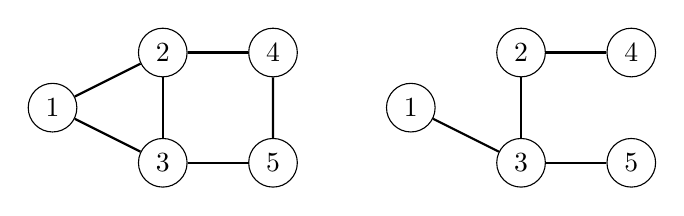
\begin{tikzpicture}[scale=0.7]
\begin{scope}
\node[draw, circle] (1) at (0,-1) {$1$};
\node[draw, circle] (2) at (2,0) {$2$};
\node[draw, circle] (3) at (2,-2) {$3$};
\node[draw, circle] (4) at (4,0) {$4$};
\node[draw, circle] (5) at (4,-2) {$5$};
\path[draw,thick,-] (1) -- (2);
\path[draw,thick,-] (1) -- (3);
\path[draw,thick,-] (2) -- (3);
\path[draw,thick,-] (4) -- (5);
\path[draw,thick,-] (2) -- (4);
\path[draw,thick,-] (3) -- (5);
\end{scope}
\begin{scope}[xshift=6.5cm]
\node[draw, circle] (1) at (0,-1) {$1$};
\node[draw, circle] (2) at (2,0) {$2$};
\node[draw, circle] (3) at (2,-2) {$3$};
\node[draw, circle] (4) at (4,0) {$4$};
\node[draw, circle] (5) at (4,-2) {$5$};
%\path[draw,thick,-] (1) -- (2);
\path[draw,thick,-] (1) -- (3);
\path[draw,thick,-] (2) -- (3);
%\path[draw,thick,-] (4) -- (5);
\path[draw,thick,-] (2) -- (4);
\path[draw,thick,-] (3) -- (5);
\end{scope}
\end{tikzpicture}
\end{center}
\caption{Verkko ja yksi sen virittävistä puista.}
\label{fig:virpuu}
\end{figure}

Jos verkko on painotettu, kiinnostava ongelma on etsiä verkon
\emph{pienin virittävä puu}.
Tämä on virittävä puu, jonka kaarten painojen summa on
mahdollisimman pieni.
Esimerkiksi kuvassa \ref{fig:pievir} on painotettu verkko ja kaksi sen virittävää puuta,
joiden painot ovat 12 ja 10.
Näistä jälkimmäinen on verkon pienin virittävä puu.

\begin{figure}
\center
\begin{center}
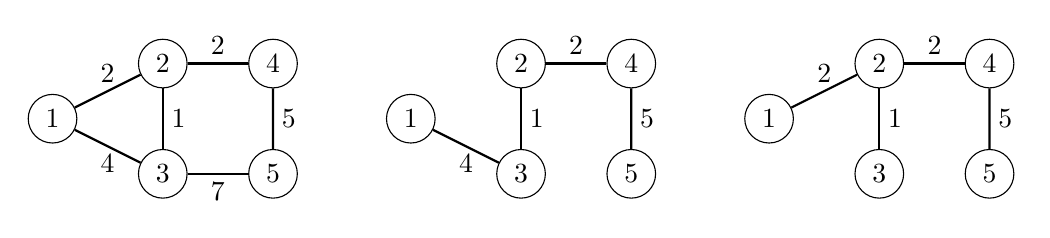
\begin{tikzpicture}[scale=0.7,label distance=-1.5mm]
\begin{scope}
\node[draw, circle] (1) at (0,-1) {$1$};
\node[draw, circle] (2) at (2,0) {$2$};
\node[draw, circle] (3) at (2,-2) {$3$};
\node[draw, circle] (4) at (4,0) {$4$};
\node[draw, circle] (5) at (4,-2) {$5$};
\path[draw,thick,-] (1) -- node[font=\small,label=above:2] {} (2);
\path[draw,thick,-] (1) -- node[font=\small,label=below:4] {} (3);
\path[draw,thick,-] (2) -- node[font=\small,label=right:1] {} (3);
\path[draw,thick,-] (4) -- node[font=\small,label=right:5] {} (5);
\path[draw,thick,-] (2) -- node[font=\small,label=above:2] {} (4);
\path[draw,thick,-] (3) -- node[font=\small,label=below:7] {} (5);
\end{scope}
\begin{scope}[xshift=6.5cm]
\node[draw, circle] (1) at (0,-1) {$1$};
\node[draw, circle] (2) at (2,0) {$2$};
\node[draw, circle] (3) at (2,-2) {$3$};
\node[draw, circle] (4) at (4,0) {$4$};
\node[draw, circle] (5) at (4,-2) {$5$};
%\path[draw,thick,-] (1) -- node[font=\small,label=above:2] {} (2);
\path[draw,thick,-] (1) -- node[font=\small,label=below:4] {} (3);
\path[draw,thick,-] (2) -- node[font=\small,label=right:1] {} (3);
\path[draw,thick,-] (4) -- node[font=\small,label=right:5] {} (5);
\path[draw,thick,-] (2) -- node[font=\small,label=above:2] {} (4);
%\path[draw,thick,-] (3) -- node[font=\small,label=below:7] {} (5);
\end{scope}
\begin{scope}[xshift=13cm]
\node[draw, circle] (1) at (0,-1) {$1$};
\node[draw, circle] (2) at (2,0) {$2$};
\node[draw, circle] (3) at (2,-2) {$3$};
\node[draw, circle] (4) at (4,0) {$4$};
\node[draw, circle] (5) at (4,-2) {$5$};
\path[draw,thick,-] (1) -- node[font=\small,label=above:2] {} (2);
%\path[draw,thick,-] (1) -- node[font=\small,label=below:5] {} (3);
\path[draw,thick,-] (2) -- node[font=\small,label=right:1] {} (3);
\path[draw,thick,-] (4) -- node[font=\small,label=right:5] {} (5);
\path[draw,thick,-] (2) -- node[font=\small,label=above:2] {} (4);
%\path[draw,thick,-] (3) -- node[font=\small,label=below:7] {} (5);
\end{scope}
\end{tikzpicture}
\end{center}
\caption{Painotettu verkko ja kaksi virittävää puuta,
joiden painot ovat $4+1+2+5=12$ ja $2+1+2+5=10$.}
\label{fig:pievir}
\end{figure}

\subsection{Kruskalin algoritmi}

Kruskalin algoritmi muodostaa verkon
pienimmän virittävän puun aloittamalla tyhjästä verkosta,
jossa on vain verkon solmut, ja lisäämällä siihen kaaria.
Algoritmi käy läpi tarjolla olevat kaaret
järjestyksessä niiden painon mukaan keveimmästä raskaimpaan.
Jokaisen kaaren kohdalla algoritmi ottaa kaaren mukaan,
jos se yhdistää kaksi eri komponenttia.
Kun kaikki komponentit on yhdistetty, pienin virittävä puu on valmis.

\begin{figure}
\center
\begin{center}
\begin{tikzpicture}[scale=0.7,label distance=-1.5mm]
\small
\newcommand\verkko[1]{
\node[draw, circle] (1) at (0,-1) {$1$};
\node[draw, circle] (2) at (2,0) {$2$};
\node[draw, circle] (3) at (2,-2) {$3$};
\node[draw, circle] (4) at (4,0) {$4$};
\node[draw, circle] (5) at (4,-2) {$5$};
\path[draw,thick,-] (1) -- node[font=\small,label=above:2] {} (2);
\path[draw,thick,-] (1) -- node[font=\small,label=below:4] {} (3);
\path[draw,thick,-] (2) -- node[font=\small,label=right:1] {} (3);
\path[draw,thick,-] (4) -- node[font=\small,label=right:5] {} (5);
\path[draw,thick,-] (2) -- node[font=\small,label=above:2] {} (4);
\path[draw,thick,-] (3) -- node[font=\small,label=below:7] {} (5);
\node at (2,-3.5) {vaihe #1};
}
\begin{scope}
\verkko{1}
\path[draw,thick,-,red,line width=2pt] (2) -- (3);
\end{scope}
\begin{scope}[xshift=6.5cm]
\verkko{2}
\path[draw,thick,-,red,line width=2pt] (2) -- (3);
\path[draw,thick,-,red,line width=2pt] (1) -- (2);
\end{scope}
\begin{scope}[xshift=13cm]
\verkko{3}
\path[draw,thick,-,red,line width=2pt] (2) -- (3);
\path[draw,thick,-,red,line width=2pt] (1) -- (2);
\path[draw,thick,-,red,line width=2pt] (2) -- (4);
\end{scope}
\begin{scope}[yshift=-5.5cm]
\verkko{4}
\path[draw,thick,-,red,line width=2pt] (2) -- (3);
\path[draw,thick,-,red,line width=2pt] (1) -- (2);
\path[draw,thick,-,red,line width=2pt] (2) -- (4);
\path[draw,thick,-,red,line width=2pt,dashed] (3) -- (1);
\end{scope}
\begin{scope}[yshift=-5.5cm,xshift=6.5cm]
\verkko{5}
\path[draw,thick,-,red,line width=2pt] (2) -- (3);
\path[draw,thick,-,red,line width=2pt] (1) -- (2);
\path[draw,thick,-,red,line width=2pt] (2) -- (4);
\path[draw,thick,-,red,line width=2pt] (4) -- (5);
\end{scope}
\end{tikzpicture}
\end{center}
\caption{Esimerkki Kruskalin algoritmin toiminnasta.}
\label{fig:kruesi}
\end{figure}

Kuva \ref{fig:kruesi} näyttää, kuinka Kruskalin algoritmi löytää pienimmän virittävän
puun esimerkkiverkossamme.
Verkon kaaret järjestyksessä keveim\-mästä raskaimpaan ovat:

\begin{center}
\begin{tabular}{rr}
kaari & paino \\
\hline
$(2,3)$ & $1$ \\
$(1,2)$ & $2$ \\
$(2,4)$ & $2$ \\
$(1,3)$ & $4$ \\
$(4,5)$ & $5$ \\
$(3,5)$ & $7$ \\
\end{tabular}
\end{center}

Algoritmi käsittelee ensin kaaren $(2,3)$.
Solmut $2$ ja $3$ ovat eri komponenteissa,
joten kaari otetaan mukaan puuhun.
Tämän jälkeen algoritmi käsittelee kaaret $(1,2)$ ja $(2,4)$,
jotka valitaan myös puuhun.
Seuraavaksi vuorossa on kaari $(1,3)$,
mutta tämä kaari ei tule puuhun,
koska solmut $1$ ja $3$ ovat jo samassa komponentissa.
Lopuksi algoritmi ottaa mukaan kaaren $(4,5)$,
jolloin pienin virittävä puu on valmis.

Voimme toteuttaa Kruskalin algoritmin tehokkaasti
käyttäen union-find-rakennetta.
Algoritmin alussa järjestämme kaaret painojärjestykseen,
missä kuluu aikaa $O(m \log m)$.
Tämän jälkeen käymme kaaret läpi, ja jokaisen kaaren
kohdalla otamme kaaren mukaan, jos se yhdistää kaksi eri komponenttia.
Tässä kuluu aikaa $O(m \alpha(n))$,
kun käytämme union-find-rakennetta.
Algoritmi vie siis yhteensä aikaa $O(m \log m)$.

\subsection{Primin algoritmi}

Primin algoritmi tarjoaa toisen lähestymistavan
pienimmän virittävän puun muodostamiseen.
Algoritmi aloittaa puun muodostamisen tilanteesta,
jossa puussa on vain yksi solmu.
Tämän jälkeen se etsii joka vaiheessa keveimmän kaaren,
jonka toinen päätesolmu kuuluu puuhun ja toinen
päätesolmu on puun ulkopuolella, ja lisää puuhun tämän kaaren.
Kun kaikki solmut on lisätty puuhun, pienin virittävä puu on valmis.

\begin{figure}
\center
\begin{center}
\begin{tikzpicture}[scale=0.7,label distance=-1.5mm]
\small
\newcommand\verkko[1]{
\node[draw, circle] (1) at (0,-1) {$1$};
\node[draw, circle] (2) at (2,0) {$2$};
\node[draw, circle] (3) at (2,-2) {$3$};
\node[draw, circle] (4) at (4,0) {$4$};
\node[draw, circle] (5) at (4,-2) {$5$};
\path[draw,thick,-] (1) -- node[font=\small,label=above:2] {} (2);
\path[draw,thick,-] (1) -- node[font=\small,label=below:4] {} (3);
\path[draw,thick,-] (2) -- node[font=\small,label=right:1] {} (3);
\path[draw,thick,-] (4) -- node[font=\small,label=right:5] {} (5);
\path[draw,thick,-] (2) -- node[font=\small,label=above:2] {} (4);
\path[draw,thick,-] (3) -- node[font=\small,label=below:7] {} (5);
\node at (2,-3.5) {vaihe #1};
}
\begin{scope}
\verkko{1}
\end{scope}
\begin{scope}[xshift=6.5cm]
\verkko{2}
\path[draw,thick,-,red,line width=2pt] (1) -- (2);
\end{scope}
\begin{scope}[xshift=13cm]
\verkko{3}
\path[draw,thick,-,red,line width=2pt] (1) -- (2);
\path[draw,thick,-,red,line width=2pt] (2) -- (3);
\end{scope}
\begin{scope}[yshift=-5.5cm]
\verkko{4}
\path[draw,thick,-,red,line width=2pt] (1) -- (2);
\path[draw,thick,-,red,line width=2pt] (2) -- (3);
\path[draw,thick,-,red,line width=2pt] (2) -- (4);
\end{scope}
\begin{scope}[yshift=-5.5cm,xshift=6.5cm]
\verkko{5}
\path[draw,thick,-,red,line width=2pt] (1) -- (2);
\path[draw,thick,-,red,line width=2pt] (2) -- (3);
\path[draw,thick,-,red,line width=2pt] (2) -- (4);
\path[draw,thick,-,red,line width=2pt] (4) -- (5);
\end{scope}
\end{tikzpicture}
\end{center}
\caption{Esimerkki Primin algoritmin toiminnasta.}
\label{fig:priesi}
\end{figure}

Kuva \ref{fig:priesi} näyttää esimerkin Primin algoritmin toiminnasta.
Voimme aloittaa puun rakentamisen mistä tahansa solmusta;
tässä esimerkissä aloitamme solmusta $1$.
Solmuun $1$ on yhteydessä kaksi kaarta $(1,2)$ ja $(2,3)$,
joista valitsemme kaaren $(1,2)$, koska se on keveämpi.
Seuraavaksi tarjolla ovat kaaret $(1,3)$, $(2,3)$ ja $(2,4)$,
joista valitsemme kaaren $(2,3)$.
Tämän jälkeen lisäämme puuhun vastaavalla tavalla kaaret
$(2,4)$, $(4,5)$, minkä jälkeen pienin virittävä puu on valmis.

Primin algoritmi muistuttaa paljon Dijkstran algoritmia.
Erona on, että Dijkstran algoritmissa valitsemme
seuraavaksi solmun, jonka etäisyys \emph{alkusolmuun} on pienin,
mutta Primin algoritmissa valitsemme solmun, jonka etäisyys
\emph{johonkin solmuun} on pienin mahdollinen.
Voimme myös toteuttaa Primin algoritmin tehokkaasti samaan
tapaan kuin Dijkstran algoritmin keon avulla,
jolloin algoritmi vie aikaa $O(m \log m)$.

\subsection{Miksi algoritmit toimivat?}

Kruskalin ja Primin algoritmit ovat ahneita algoritmeja:
ne lisäävät joka askeleella keveimmän mahdollisen kaaren puuhun.
Miksi on varmaa, että algoritmit tuottavat pienimmän virittävän
puun joka tilanteessa?

Voimme ajatella asiaa näin: 
Jos meillä on kaksi solmua $a$ ja $b$, jotka ovat eri komponenteissa,
meidän on yhdistettävä ne jotenkin samaan komponenttiin algoritmin aikana.
Jos kevein saatavilla oleva kaari on solmujen $a$ ja $b$ välillä,
meidän kannattaa valita se, koska muuten joutuisimme yhdistämään komponentit
käyttäen raskaampaa kaarta.

Tarkastellaan esimerkkinä Kruskalin algoritmin alkua:
mitä tapahtuu, jos emme valitse puuhun keveintä kaarta?
Kuvassa \ref{fig:pietod} näkyy kuvitteellinen tilanne,
jossa katkoviivoilla esitetty pienin virittävä puu ei sisällä
keveintä kaarta $(2,3)$, jonka paino on 1.
Ei ole kuitenkaan mahdollista, että tämä olisi todellisuudessa
pienin virittävä puu, koska voisimme vaihtaa jonkin puun kaaren
kaareen $(2,3)$ ja saada pienennettyä puun painoa.

Tämä tarkoittaa, että on varmasti turvallinen ratkaisu valita
kevein kaari puuhun Kruskalin algoritmin alussa.
Vastaavasti voimme perustella, miksi seuraavaksi kannattaa
valita seuraavaksi kevein kaari jne.

TODO parempi todistus?


\begin{figure}
\center
\begin{center}
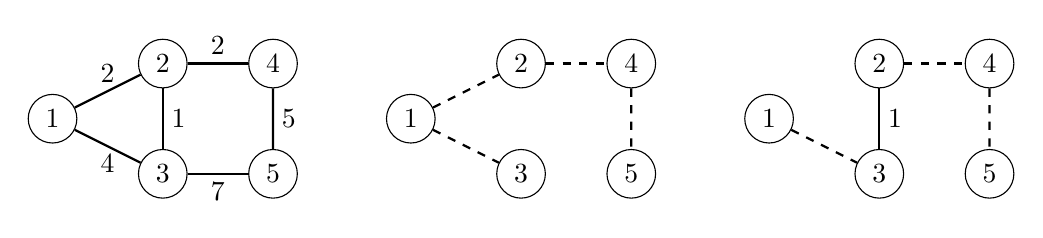
\begin{tikzpicture}[scale=0.7,label distance=-1.5mm]
\begin{scope}
\node[draw, circle] (1) at (0,-1) {$1$};
\node[draw, circle] (2) at (2,0) {$2$};
\node[draw, circle] (3) at (2,-2) {$3$};
\node[draw, circle] (4) at (4,0) {$4$};
\node[draw, circle] (5) at (4,-2) {$5$};
\path[draw,thick,-] (1) -- node[font=\small,label=above:2] {} (2);
\path[draw,thick,-] (1) -- node[font=\small,label=below:4] {} (3);
\path[draw,thick,-] (2) -- node[font=\small,label=right:1] {} (3);
\path[draw,thick,-] (4) -- node[font=\small,label=right:5] {} (5);
\path[draw,thick,-] (2) -- node[font=\small,label=above:2] {} (4);
\path[draw,thick,-] (3) -- node[font=\small,label=below:7] {} (5);
\end{scope}
\begin{scope}[xshift=6.5cm]
\node[draw, circle] (1) at (0,-1) {$1$};
\node[draw, circle] (2) at (2,0) {$2$};
\node[draw, circle] (3) at (2,-2) {$3$};
\node[draw, circle] (4) at (4,0) {$4$};
\node[draw, circle] (5) at (4,-2) {$5$};
\path[draw,thick,-,dashed] (1) -- (2);
\path[draw,thick,-,dashed] (1) -- (3);
\path[draw,thick,-,dashed] (4) -- (5);
\path[draw,thick,-,dashed] (2) -- (4);
\end{scope}
\begin{scope}[xshift=13cm]
\node[draw, circle] (1) at (0,-1) {$1$};
\node[draw, circle] (2) at (2,0) {$2$};
\node[draw, circle] (3) at (2,-2) {$3$};
\node[draw, circle] (4) at (4,0) {$4$};
\node[draw, circle] (5) at (4,-2) {$5$};
\path[draw,thick,-,dashed] (1) -- (3);
\path[draw,thick,-] (2) -- node[font=\small,label=right:1] {} (3);
\path[draw,thick,-,dashed] (4) -- (5);
\path[draw,thick,-,dashed] (2) -- (4);
\end{scope}
\end{tikzpicture}
\end{center}
\caption{Pienin virittävä puu sisältää varmasti kaaren $(2,3)$,
koska muuten voisimme pienentää puun painoa valitsemalla sen.}
\label{fig:pietod}
\end{figure}
